\subsection{PCAPS (Salt Lake Valley) Plots}
\begin{figure} 
\centering 
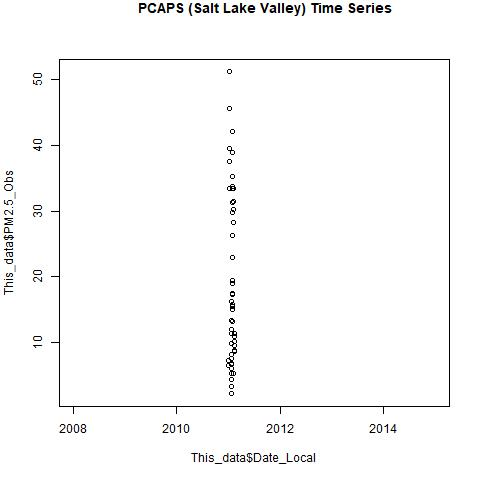
\includegraphics[width=0.77\textwidth]{Code_Outputs/PCAPS_time_series.jpg} 
\caption{\label{fig:PCAPSTS}PCAPS (Salt Lake Valley) time series. There are 0 data points (out of 59) with concentrations greater than 200 ug/m3} 
\end{figure} 
 

\begin{figure} 
\centering 
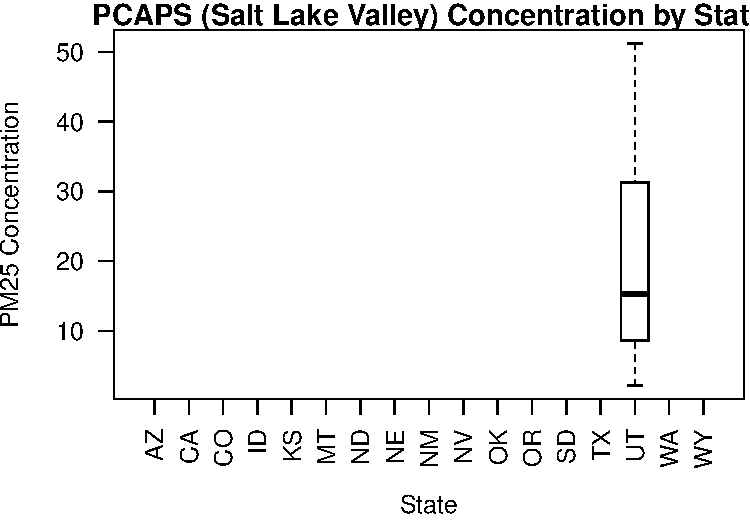
\includegraphics[width=0.77\textwidth]{Code_Outputs/PCAPS_state_boxplots.pdf} 
\caption{\label{fig:PCAPSBP}PCAPS (Salt Lake Valley) box plots.} 
\end{figure} 
 

\begin{figure} 
\centering 
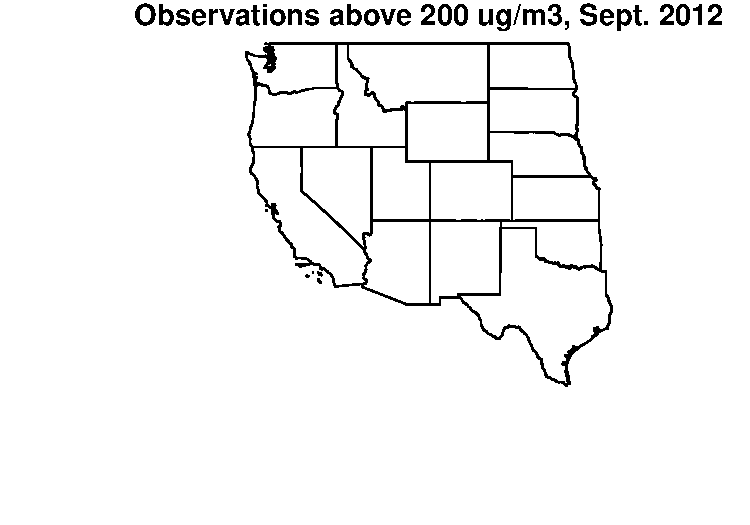
\includegraphics[width=0.77\textwidth]{Code_Outputs/PCAPSSep2012High_map.pdf} 
\caption{\label{fig:PCAPSS12}PCAPS (Salt Lake Valley) map of locations with PM2.5 above 200 ug/m3 during Sept 2012.} 
\end{figure} 
 
